% This is LLNCS.DEM the demonstration file of
% the LaTeX macro package from Springer-Verlag
% for Lecture Notes in Computer Science,
% version 2.4 for LaTeX2e as of 16. April 2010
%
\documentclass{llncs}
% % % % % % % % % % % % % % % % % % % %
% For Russian uncomment the following lines
%\usepackage[utf8x]{inputenc}
%\usepackage[russian]{babel}
% \def\keywordname{{\bf Ключевые слова:}}%
% % % % % % % % % % % % % % % % % % % % 
\usepackage{graphicx}
\usepackage{comment}
%\usepackage[title]{appendix}
\begin{document}
%
\title{Telling the story of best friends: marker rank statistics}
%
\titlerunning{Best friends}  
% abbreviated title (for running head)
%                                     also used for the TOC unless
%                                     \toctitle is used
%
\author{Alexander Favorov\inst{1}\textsuperscript,\inst{2}
\and Vera Mukhina \inst{2,3} \and Vasiliy Ramensky \inst{4}
\and Andrey Mironov \inst{3}\textsuperscript,\inst{5}}
%
\authorrunning{A. Favorov et al.} % abbreviated author list (for running head)
%
%%%% list of authors for the TOC (use if author list has to be modified)
\tocauthor{Alexander Favorov, Vera Mukhina, Vasiliy Ramensky, and Andrey Mironov}
%
\institute{
Johns Hopkins University School of Medicine, \\ Baltimore, MD 21205, USA,
\and
Vavilov Institute of General Genetics, RAS, \\ Moscow, 119333, Russia, 
\email{favorov@sensi.org}
\and
Institute for Information Transmission Problems, RAS, \\ Moscow,  127994, Russia
\and
National Health and Research Center of Preventive Healthcare, \\ Moscow, 101990, Russia
\and
Faculty of Bioengineering and Bioinformatics, MSU, \\ Moscow, 119992, Russia
}

\maketitle              % typeset the title of the contribution

\newcommand{\tag}{tag}
\newcommand{\cloud}{cloud}
\newcommand{\T}{T}
\newcommand{\C}{C}
\newcommand{\tl}{t}
\newcommand{\cl}{c}

\begin{abstract}


Suppose we have a set of {\tag}s and a set of fuzzy set of {\tag}s, which we will refer to as {\cloud}s, and a we have the {\tag}-to-{\cloud} relation quantified as a scalar for each $\left( {\tag},{\cloud}\right)$ pair. An example is: {\tag}s are genes, {\cloud}s are gene expression patterns, and the scalars are loads of the genes in the patterns. Sometimes, observation that a gene is expressed implies expression of a particular pattern (the simplest case is: the gene has nonzero load only in that pattern). If so, we say that the gene marks the pattern. Here we describe a statistical test that identify pairs of a marker {\tag} and the marked {\cloud}. The test is based on rank statistics and it does not rely on propositions about the distribution of the relation quantity. The marked {\cloud} is referred to as the {\tag}'s best friend, and the test is named "the best friends test" or "the gene's best friends test". The statistics is naturally expand to the case when a {\tag} selects (separates) a subset of {\cloud}s, thus having more than one best friend. The code (currently, only R) is available at \url{https://github.com/favorov/best-friends}
\keywords{best friends, gene's best friends, specific gene regulation, pattern marker, rank statistics, marker feature, marked entity}
\end{abstract}
%
\section{Introduction: friends and markers}

There is a simple intuition of what does it mean to be a friend. A friend of Augustus cares about Augustus more than about other persons. And, if one sees Augustus, it makes sense to infer to see friends(s) of Augustus also. Lets’s try to translate it to statistical inferences.

Let's picture a set of genes and their loads in expression patterns. Each pattern describes the expression of the genes in some process. Sometimes, we can conclude that a pattern is expressed from expression of a single gene. The simplest case that allows this inference is when the gene has nonzero load in only one pattern. The situation when other loads are just relatively small, also fits the inference. We will refer to the gene as marker gene and to the pattern as the best friend of the gene. We want to identify the marker genes and their best friends given the load matrix.

We formulated \cite{best_friends:2015} the similar task in a symmetric form on gene expression data as searching for genes that are best friends of genes. Best friend of a gene $G_i$ is another gene $G_j$ that is expressed concertedly with the gene $G_i$, while other genes $G_k, k\neq i, k \neq j$ are (almost) not. The best friend is unique, while one gene can be the best friend for more than one gene. The solution we proposed (rank backwards ranking) showed the putative pairs of marker and its best friend, but it did not provide either statistical measure or an effect size estimate. Later, the problem was also formulated in an asymmetric setup \cite{patternmarkers:2017} for genes and expression patterns, and the solution was to scale each gene's loads to $max((\mbox{all loads for this gene})==1$ and calculate the Euclidean distance between the scaled vector of loads and the ideal $(0,0,...,1,...0$). The less the distance is, the better the marker is. 

Let's make a generalisation. We have entities and features and a matrix that show how strong is a feature ascribed to an entity. We want to identify those features that reliably and uniquely identify an entity. Let's call the feature the entity's marker and let's call the entity the feature's best friend. Here, we describe a rank test identifying significant pairs of marker feature and its best friend entity.

\begin{comment}
\subsection{ex-abstract}
Suppose we have set of {\tag}s $\T$ and a set of {\cloud}s $\C$ of this {\tag}s with some fuzzy membership, e.g. there is a numeric measure of how an {\tag} is represented in a {\cloud} $A(\tl,\cl)$ for each pair $(\tl,\cl):\tl \in \T, \cl \in \C$. The higher the $A(\tl,\cl)$ value is, the more the {\tag} $\tl$ is involved in the {\cloud} $\cl$. The absence of the {\tag} in the {\cloud} is shown by the value that is minimal for the {\cloud}.

An example that is easy to think about is: genes are {\tag}s and their groups under regulation by same transcription factors (TF’s) form {\cloud}s, and A shows the strength of the regulation. We look at a gene and we want to know whether a TF is its friend, i.e. whether the TF specifically prefers (regulates) the gene. The na\"ive idea is to look for a TF that the gene is the most sensitive for. Still, it’s possible that this TF is the strongest for the most of the genes. Sometimes, it is what we want to find, but now we want to answer other questions, namely, what TF is the most specific factor for the gene and is the specificity enough to say that is does not look like a random outcome?

Sometimes, the {\cloud}s are in in one-to-one relation with the {\tag}s, e.g. each {\cloud} is a set of {\tag}s, which are neighbours of {\tag} in some graph. For this example, A is a weighted adjacency matrix of this graph. The friendship terminology emerges naturally from this case. The friendship relation itself is asymmetric: a friend cares about Augustus, while Augustus does not.
\end{comment}

%
\section{Method}
\subsection{Ranking}

How does the friendship of a community to one of the elements looks like in terms of the $A$ values? The rank of the element in the friendly community is to be higher than in other communities and the difference is to be very unlikely to be obtained by chance. In other words, for every $\tl_i \in T$, and $\cl_j \in C$, let $A(\tl_i, \cl_j) = a^i_{j}$.

% Rank over $t_i$: $a^{(i)}_{j}$\\
% Rank over $t_i$ and $c_j$: $a^{(i)}_{(j)}$

$j$ is fixed: define $r_{\cl_j}( a^i_{j}) = (i)_j$,\\ $r_{\tl}( a^{(i)}_{j}) = a^{(i)}_{(j)}$




%=========
Let's say we have an $A_{ij} = A(\tl_i, \cl_j)$ - matrix that represent the strength of relation between $k = |T|$ tags and $n = |C|$ clouds. We want to identify all entities that are preferably selected (marked) by one or more features. Such a feature is a marker for the entity, and the entity is the best friend for the fea fture.
First, we rank all the features by its $A_{ij}$ for each entity $j$, so obtaining $R_{ij}= \text xrm{rank of } P_{ij} \textrm{ in } P_{*j}$. Then, we scale $R$ into $[0..1]$ : $r_{ij}={R_{ij}}/{k}$. To be specific, we suppose that the ranking is ascending, the smaller is the rank, the stronger is the relation.

\subsection{Single marker rank statistics}
For each feature $i,i=1..k$, we obtain a vector $r_{ij}, j=1..n$. There are normalised ranks of the feature in different entities, in the a null hypothesis they are uniformly i.i.d. in [0,1]. Let's create a rank statistics $u_i$ by ordering their values. If a feature is a unique marker for an entity, the entity corresponds to the first  value $u_1$. Let's use the difference $u_2-u_1$ as a measure of uniqueness (quality of the marker). Indeed, if we see that the difference is significantly higher than we can expect if null hypothesis holds, we can conclude that the feature unexpectedly prefer the entity, so it is a marker (and the entity is its best friend). Similarly to the density estimation for each $u_i$ (see, e.g. \cite{Gut:2009}) we estimate the probability to observe the difference $u_2 - u_1 \ge t$. 

First, the whole n-dimension (nD) volume of ranked variables $u_1 .. u_n$ is:
\begin{eqnarray*}
V = &\displaystyle \int_0^1\int_{u_1}^1\int_{u_2}^1\int_{u_3}^1...\int_{u_{n-1}}^1 du_n....du_4 du_3 du_2 du_1 =  \frac{1}{n!}
\end{eqnarray*}
see eq. \ref{eq:volume} for details.

Let's denote the p-value for the observation $t=u_2-u_1$ as $p_1(t)$. $p_1(t)$ is the ratio of nD, that is limited by $t<=u_2-u_1$ condition, and $V$.

\begin{eqnarray*}
p(t) = & \displaystyle\frac{1}{V} \displaystyle \int_0^{1-t}\int_{{u_1}+t}^1\int_{u_2}^1\int_{u_3}^1...\int_{u_{n-1}}^1 du_n....du_4 du_3 du_2 du_1 = (1-t)^n
\end{eqnarray*}
see eq. \ref{eq:p_1} for details.

After the correction this p-value for multiple hypothesis testing (each feature provides its own null hypothesis), we identify the statistically significant pairs of a feature (marker) and entity (its best friend).

\subsection{Multiple marker rank statistics}
Now, let's suppose that an entity has more than one features, that almost equally good marks it, for example, two genes has nonzero load in a pattern. The pattern is the best friend for both of them, and each of them or their combination is a unique marker for the pattern, but the single marker rank statistics cannot find them, for the distance $u_2-u_1$ is quite low: the markers are almost equally good.

\subsection*{Notes and comments}

For a symmetric case, sometimes it makes sense to remove the main diagonal before ranking not to obtain trivial self-relations.

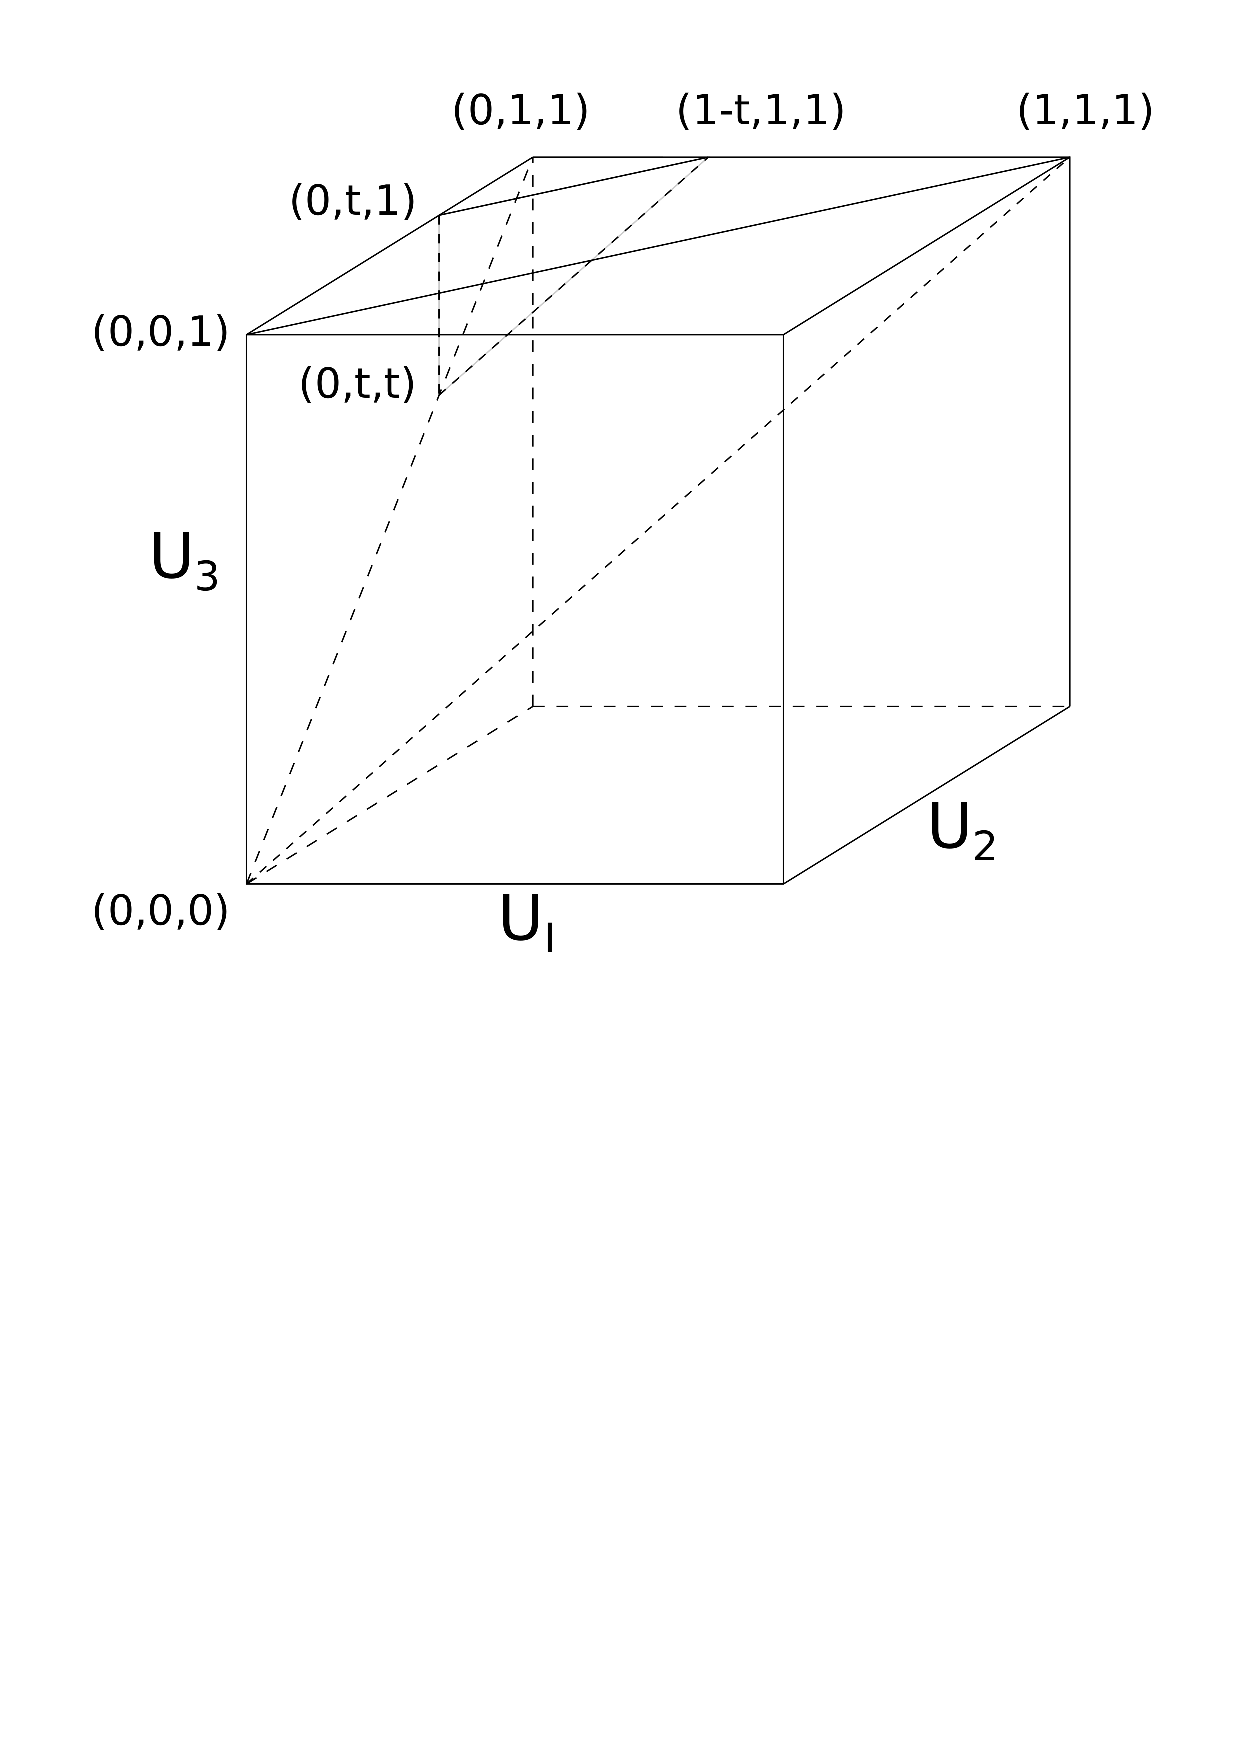
\includegraphics[scale=.5,trim=0 10cm 0 0, clip=true]{rank3d-nocolour}

The figure explains the probability estimation for the $n=3$ case. The rank statistics probability density is $3!=6$ and it uniformly scattered in (0,0,0), (0,0,1), (0,1,1), (1,1,1) tetrahedron. The $u_2 - u_1 \ge t$ condition holds only in the (0,t,t), (0,t,1), (0,1,1), (1-t,1,1) small tetrahedron.

To assess the p-value for a feature $i$, we do not need to rank the whole $r_{ij}, j=1..n$ vector to build the rank statistics $u_j$; we actually need only the $t$ value, so it is enough to find the maximal and the second values of $r_{ij}$.

\section{Discussion}

We formulated a statistical test that to detest reliable pairs of marker feature and the marked entity. Nevertheless the formulation of the problem looks abstract, its solution provides numerous straightforward application. The motivating example we started with was to detect the marker genes for expression patterns. The patterns could be obtained from the CoGAPS (scCoGAPS) \cite{Fertig_2016} or other matrix factorisation method \cite{Stein_2018}. The identification of the marker genes can critically simplify biological interpretation. If the matrix is the amplitude component from  the decomposition, the marker time points (or, the marker cells for scCoGAPS) can also be very informative for analysis. If the matrix contains the expression correlation for two gene sets, annotated best friends of an non-annotated gene extend the existing annotation.

\section{Conflict of interest}
Authors declares no conflict of interest.

\section{Acknowledgements}
AF acknowledges support by National Institutes of Health (NIH) P30CA006973 and 1U01CA253403-01, Russian Foundation for Basic Research (RFBR) 17-00-00208, the Russian Academy of Sciences Project 0112-2019-0001; VR acknowledges support from RFBR 20-54-12008; AM acknowledges support from RFBR 20-04-00459.

\bibliography{gene-best-friends}

\bibliographystyle{splncs03}
%\begin{subappendices}

\newcommand{\beginsupplement}{%
        \setcounter{table}{0}
        \renewcommand{\thetable}{S\arabic{table}}%
        \setcounter{figure}{0}
        \renewcommand{\thefigure}{S\arabic{figure}}
        \setcounter{equation}{0}
        \renewcommand{\theequation}{S\arabic{equation}}%
     }
\section*{Supplement}
\beginsupplement

%\renewcommand{\thesection}{\Alph{section}}%
% or try \arabic{section}
For an integer $m$,
\begin{eqnarray}
&\displaystyle \int_a^b\left(b-x\right)^{m-1}dx=
%-\displaystyle \int_0^{1-a}v^{n-1}dv=
\displaystyle \frac{\left(b-a\right)^m}{m}  \label{eq:intab}
\end{eqnarray} 
%\begin{eqnarray}
%&\displaystyle \int_a^1\left(1-x\right)^{m-1}dx=
%-\displaystyle \int_0^{1-a}v^{n-1}dv=
%\displaystyle \frac{\left(1-a\right)^m}{m}  \label{eq:right}
%\end{eqnarray} 
%\begin{eqnarray}
%&\displaystyle \int_0^b\left(b-x\right)^{m-1}dx=\displaystyle \frac{b^m}{m}  \label{eq:left}
%\end{eqnarray}
Applying \ref{eq:intab} recursively from $u_n$ until $u_1$: 
\begin{eqnarray}
V = &\displaystyle \int_0^1\int_{u_1}^1\int_{u_2}^1\int_{u_3}^1...\int_{u_{n-1}}^1 du_n...du_4 du_3 du_2 du_1 = \nonumber \\ 
&\displaystyle \frac{1}{(n-3)!}\int_0^1\int_{u_1}^1\int_{u_2}^1 \left( 1-u_3 \right)^{n-3}du_3 du_2 du_1 = \nonumber \\
&\displaystyle \frac{1}{(n-2)!}\int_0^{1-t}\int_{{u_1}+t}^1\left( 1-u_2 \right)^{n-2} du_2 du_1 = \nonumber \\
&\displaystyle \frac{1}{(n-1)!} \int_0^1\left( 1-u_1 \right)^{n-1} du_1 = \frac{1}{n!} \label{eq:volume}
\end{eqnarray} 
\begin{eqnarray}
& p_1(t) =  \displaystyle \frac{1}{V}\displaystyle \int_0^{1-t}\int_{{u_1}+t}^1\int_{u_2}^1\int_{u_3}^1...\int_{u_{n-1}}^1 du_n...du_2 du_1 =  \nonumber \\ 
%&\displaystyle \frac{n!}{(n-3)!}\int_0^{1-t}\int_{{u_1}+t}^1\int_{u_2}^1 \left( 1-u_3 \right)^{n-3}du_3 du_2 du_1 =  \nonumber \\
&\displaystyle \frac{n!}{(n-2)!}\int_0^{1-t}\int_{{u_1}+t}^1\left( 1-u_2 \right)^{n-2} du_2 du_1 =  \nonumber \\
&\displaystyle n \int_0^{1-t}\left( 1-t-u_1 \right)^{n-1} du_1 = (1-t)^n \label{eq:p_1}
\end{eqnarray}
\begin{eqnarray}
& p_k(t) = \displaystyle \frac{1}{V}\displaystyle \int_0^{1-t}\int_{{u_1}}^{1-t}...\int_{u_{k-1}}^{1-t}\int_{u_k+t}^1...\int_{u_{n-1}}^1 du_n... du_1 =  \nonumber \\ 
& \displaystyle \frac{n!}{(n-k-1)!}\displaystyle \int_0^{1-t}\int_{{u_1}}^{1-t}...\int_{u_{k-1}}^{1-t}\int_{u_k+t}^1 \left( 1-u_{k+1} \right)^{n-k-1} du_{k+1}...du_1 =  \nonumber \\
& \displaystyle \frac{n!}{(n-k)!}\displaystyle \int_0^{1-t}\int_{{u_1}}^{1-t}...\int_{u_{k-1}}^{1-t} \left( 1-t-u_{k} \right)^{n-k} du_k...du_1 =  \nonumber \\
& \displaystyle \frac{n!}{(n-k+1)!}\displaystyle \int_0^{1-t}\int_{{u_1}}^{1-t}...\int_{u_{k-2}}^{1-t} \left( 1-t-u_{k-1} \right)^{n-k+1} du_{k-1}...du_1 =  \nonumber \\
& \displaystyle n \int_0^{1-t}\left( 1-t-u_1 \right)^{n-1} du_1 = (1-t)^n \label{eq:p_k}
\end{eqnarray}
%\end{subappendices}

\end{document}


